\documentclass[utf8,xcolor=table]{beamer}

\usepackage[T2A]{fontenc}
\usepackage[utf8]{inputenc}
\usepackage[english,russian]{babel}
\usepackage{minted}
\usepackage{ulem}
\usepackage{cmap}
\usepackage{multirow}

\hypersetup{colorlinks,linkcolor=blue,urlcolor=blue}

\mode<presentation>{
	\usetheme{CambridgeUS}
}

\renewcommand{\t}[1]{\ifmmode{\mathtt{#1}}\else{\texttt{#1}}\fi}

\title{Функциональное программирование}
\author{Егор Суворов}
\institute[СПб АУ]{Курс <<Парадигмы и языки программирования>>, подгруппа 3}
\date[20.11.2017]{Понедельник, 20 ноября 2017 года}

\setlength{\arrayrulewidth}{1pt}

\begin{document}

\begin{frame}
\titlepage
\end{frame}

\begin{frame}{План занятия}
	\tableofcontents
\end{frame}

\section{Функциональное программирование}
\subsection{Примеры на Python}

\begin{frame}
	\tableofcontents[currentsection,currentsubsection]
\end{frame}

\subsection{Императивное программирование}
\begin{frame}{Императивное программирование}
	Руководствуемся следующим принципом:
	\begin{exampleblock}{Определение}
		Алгоритм "--- набор инструкций, описывающих порядок действий исполнителя для достижения некоторого результата
	\end{exampleblock}
	\begin{itemize}
		\item В императивном стиле код программы описывает \textit{как} надо достигать результата.
		\item Есть постоянно изменяющееся состояние программы (например, переменные).
		\item Хорошо ложится на <<железо>>: оно действительно меняет состояние памяти.
	\end{itemize}
\end{frame}

\begin{frame}{Что такое <<действие>>?}
    Можно работать на разных уровнях абстракции:
	\begin{itemize}
		\item Команда процессора: <<возьми значение из ячейки памяти с таким номером>>
		\item Вычисление арифметического выражения
		\item Конструкции управления \t{if}/\t{for}/\t{while}
		\item Вызовы функций
	\end{itemize}
\end{frame}

\begin{frame}{Функциональное программирование}
	\begin{exampleblock}{Определение}
		Алгоритм "--- это \textit{чистая} математическая функция от нескольких аргументов.
	\end{exampleblock}
	\begin{itemize}
		\item Как решение задачи на курсе алгоритмов.
		\item Основное свойство "--- \textit{чистота} функций; результат вычисления зависит только от аргументов функции.
		\item Ни слова про состояние программы или порядок вычислений.
		\item Остальные свойства выводятся из чистоты:
			\begin{itemize}
				\item Порядок вычислений неважен.
				\item Состояние программы не может влиять на работу функций.
				\item Например, функция не может читать из глобальных переменных.
			\end{itemize}
	\end{itemize}
\end{frame}

\begin{frame}{Побочные эффекты}
	\begin{itemize}
		\item То, что происходит в функции помимо вычисления значения, называется \textit{побочным эффектом}.
		\item Результаты всех функций зависят только от аргументов $\iff$ у функций нет побочных эффектов.
		\item В <<идеально чистых>> языках запрещены не только функции с побочными эффектами, но любые побочные эффекты вообще.
		\item В частности, запрещено иметь изменяемое состояние "--- переменные.
		\item Никаких гонок данных.
		\item Непонятно, как тогда делать ввод-вывод "--- это точно побочный эффект.
		\item Идеально чистые языки бесполезны, все в той или иной степени <<загрязнены>>.
	\end{itemize}
\end{frame}

\begin{frame}[fragile]{Задача о рюкзаке, императивное решение}
\begin{minted}{cpp}
int maxSumCost = 0;
void solve(int i, int weight, int cost) {
  maxSumCost = max(maxSumCost, cost);  // Не чистая
  if (i == n) return;
  solve(i + 1, weight, cost);
  if (weight >= ws[i]) {
    solve(i + 1, weight - ws[i], cost + cs[i]);
  }
}
\end{minted}
\end{frame}

\begin{frame}[fragile]{Задача о рюкзаке, чистая функция-1}
\begin{minted}{cpp}
int solve(int i, int weight, int cost) {
  if (i == n) return cost;
  int ans = solve(i + 1, weight, cost);
  if (weight >= ws[i]) {
    ans = max(ans, solve(i + 1,
                         weight - ws[i],
                         cost + cs[i]));
  }
  return ans;
}
\end{minted}
\end{frame}

\begin{frame}[fragile]{Задача о рюкзаке, чистая функция-2}
\begin{minted}{cpp}
int solve(int i, int weight, int cost) {
  if (i == n) return cost;
  if (weight < ws[i]) return solve(i + 1, weight, cost);
  return max(
    solve(i + 1, weight, cost),
    solve(i + 1, weight - ws[i], cost + cs[i])
  );
}
\end{minted}
\end{frame}

\begin{frame}[fragile]{Задача о рюкзаке, чистая функция-3}
\begin{minted}{cpp}
int solve(int i, int weight) {
  if (i == n) return 0;
  if (weight < ws[i]) return solve(i + 1, weight);
  return max(
    solve(i + 1, weight),
    solve(i + 1, weight - ws[i]) + cs[i]
  );
}
\end{minted}
\end{frame}

\begin{frame}[fragile]{Императивная работа с массивом}
\begin{minted}{python}
lst = [5, 10, 15, 10, 20]
partialSums = []
smallPrefix = []
s = 0
for x in lst:
    if x >= 10:
        s += x
        partialSums.append(s)
    if x <= 10:
        smallPrefix.append(x)

for i in range(len(lst)):
    lst[i] *= 2
\end{minted}
\end{frame}

\begin{frame}[fragile]{Функциональная работа с массивом}
\begin{minted}{python}
import itertools
lst = [5, 10, 15, 10, 20]
partialSums = list(itertools.accumulate(
  # filter - "функция высшего порядка"
  filter(lambda x: x >= 10, lst)
))
smallPrefix = list(
  # takewhile- "функция высшего порядка"
  itertools.takewhile(
    lambda x: x <= 10, lst)
)
lst = [x * 2 for x in lst]
# lst = map(lambda x: x * 2, lst)
\end{minted}
\end{frame}

\subsection{Жизнь без переменных}

\begin{frame}{Haskell}
	\begin{itemize}
		\item Haskell "--- чистый функциональный язык программирования.
		\item Компилируемый, статически типизирован, \textit{очень} мощная система типов.
		\item Есть огромное число библиотек.
		\item Очень чистый по сравнению с остальными языками вроде OCaml.
		\item Помимо функциональной чистоты имеет огромное количество интересных особенностей.
		\item На нём действительно можно писать код.
		\item Стандартный компилятор "--- GHC (Glasgow Haskell Compiler).
		\item Рекомендуется использовать в составе \href{https://www.haskell.org/platform/}{Haskell Platform}.
	\end{itemize}
\end{frame}

\begin{frame}{Демонстрация}
	\begin{enumerate}
		\item Демо: арифметика, простые типы, сравнения, списки, работа со списками, list comprehension.
		% 01-01-demo.hsi
		\item Упражнение: как найти все Пифагоровы тройки ($x^2 + y^2 = z^2$) при $1 \le x, y, z \le 10$?
		\item Интерпретатор \t{ghci} не поддерживает многострочные определения функций.
		\item Поэтому с некоторого момента лучше набирать код в файле, подгружая его в интерпретатор:
			\begin{itemize}
				\item \t{:load file.hs} (\t{:l file.hs}) компилирует \t{file.hs} и подгружает определения в интерпретатор.
				\item \t{:reload} перекомпилирует и переподключит все файлы.
			\end{itemize}
		\item Демо: функции, комментарии, определения функций <<и>>, <<или>>, <<сумма двух чисел>>.
		% 01-02-funcs.hs
	\end{enumerate}
\end{frame}

\begin{frame}{Жизнь без циклов}
	Упражнения на Python:
	\begin{itemize}
		\item Как посчитать сумму чисел в списке, если нет переменных и циклов?\pause
		\item Функция \t{sum}.\pause
		\item Как посчитать сумму квадратов чисел? \pause
		\item Определить лямбда-функцию для возведения в квадрат и применить \t{map} с \t{sum}.\pause
		\item Какие вообще операции со списками мы ещё не умеем делать без циклов? \pause
		\item В которых элементы влияют друг на друга.
	\end{itemize}
	Демо: то же самое на Haskell.
	% 01-03-exercise.hs
\end{frame}

\begin{frame}[fragile]{Не самый хороший императивный код}
	% 01-04-avg-len-imp.py
\begin{minted}{python}
s = "hello good world"
a = 0
b = 0
flag = False
for c in s + " ":
    if c == " ":
        if flag:
            a += 1
        flag = False
    else:
        b += 1
        flag = True
print(b / a)
\end{minted}
	И что тут происходит?
\end{frame}

\begin{frame}{Моя реакция на такой код}
	\begin{center}
		
\includegraphics{wtf-panda.png}
	\end{center}
\end{frame}

\begin{frame}[fragile]{На самом деле}
	Это вычисление средней длины слова в строке.

	Чем плохо?
	\begin{itemize}
		\item 11 строк на такое простое действие.
		\item Есть сложный инвариант.
		\item Тестировать сложно: надо подбирать специальную строку, на которой отличается средняя длина слов (а не просто воспроизводится баг).
	\end{itemize}
\end{frame}

\begin{frame}{Функциональное решение}
	\begin{itemize}
		\item Как записать то же самое функционально на Python? \pause
		\item Предполагаем, что есть функции \t{avg}, \t{map}, \t{split}. \pause
		\item \t{avg(map(len, "hello world".split()))} \pause
		% 01-05-avg-len-func.py
		\item Тут что-то сложное делает только функция split.
		\item Обычно \t{split()} пишут <<императивно>>, а всю последующую обработку "--- <<функционально>>.
		\item Таким образом императивная сложность изолирована, все кусочки можно тестировать по отдельности.
		\item Опять ввели абстракцию: три встроенные функции.
		\item Оказывается, что <<необходимых кирпичиков>> не так много.
	\end{itemize}
\end{frame}

\begin{frame}{Моя реакция на функциональный код}
	\begin{center}
		
\includegraphics[scale=0.3]{satisfied-seal.jpg}
	\end{center}
\end{frame}

\begin{frame}{Рандом в функциональном стиле}
	\begin{center}
		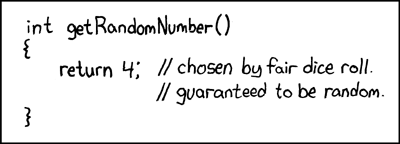
\includegraphics[scale=0.3]{random_number.png}
	\end{center}
\end{frame}

\section{Интересный Haskell}
\subsection{Рекурсия}

\begin{frame}
	\tableofcontents[currentsection,currentsubsection]
\end{frame}

\begin{frame}[t,fragile]{Упражнения на рекурсию}
	% 02-01-rec.hs
	\begin{tabular}{p{0.45\linewidth}p{0.45\linewidth}}
	\centering
	Факториал:
\begin{minted}{haskell}
fac 0 = 1
fac n = n * fac (n - 1)
\end{minted}
	&
	Степень двойки: \pause
\begin{minted}{haskell}
powerOfTwo 0 = 1
powerOfTwo n = 2 *
    powerOfTwo (n - 1)
\end{minted}
	\end{tabular}
	\vspace{-10pt}

	Числа Фибоначчи: \pause
\begin{minted}{haskell}
fib n = fib' 0 1 n
fib' f1 f2 0 = f1
fib' f1 f2 n = fib' f2 (f1 + f2) (n - 1)
\end{minted}
	\begin{itemize}
		\item Функции могут содержать апостроф
		\item Функции всегда должны начинаться с маленькой буквы.
		\item Мы увидели \textit{pattern matching}:
			\begin{itemize}
				\item Вместо \t{if} пишем <<шаблон>> для аргумента функции.
				\item Шаблонов может быть несколько, они проверяются сверху вниз.
				\item Приближает нас к математической нотации, избавляет от if'ов.
				\item Очень популярно в функциональных языках.
			\end{itemize}
	\end{itemize}
\end{frame}

\begin{frame}[fragile]{If не нужен}
	% 02-02-if.hs
	% 02-03-no-if.hs
\begin{minted}{haskell}
-- If
fac n = if n == 0
        then 1
        else n * fac (n - 1)
-- Pattern matching
fac 0 = 1
fac n = n * fac (n - 1)
-- If
facTwo n = if n <= 1
           then 1
           else n * facTwo (n - 2)
-- Guards
facTwo n | n <= 1    = 1
         | otherwise = n * fac (n - 2)
\end{minted}
\end{frame}

\begin{frame}[t,fragile]{Жизнь без циклов}
	Как теперь написать функцию \t{sum}?
	% 02-04-sum1.hs
\begin{minted}{haskell}
sum' (x:xs) = x + sum' xs
sum' _ = 0
\end{minted}
	\begin{itemize}
		\item Иногда можно делать сложный pattern matching вроде \t{x:xs} (список, первый элемент которого "--- \t{x}, а хвост "--- \t{xs}).
		\item Шаблоны проверяются сверху вниз, выбирается первый подходящий.
		\item Вместо имени переменной можно написать \t{\_}.
	\end{itemize}
\end{frame}

\begin{frame}[fragile]{Неявный инвариант}
	Если в императивной программе есть цикл "--- то можно вынести одну итерацию этого цикла в функцию и сделать рекурсию вместо цикла:

	\begin{tabular}{p{0.35\linewidth}p{0.55\linewidth}}
		\centering
		% 02-04-sum2.py
		% 02-04-sum2.hs
		Python & Haskell \\
\begin{minted}{python}
def sum(xs):
    a = 0
    for x in xs:
        a += x
    return a
\end{minted}
		&
\begin{minted}{haskell}
sum' xs = sum'' 0 xs
sum'' a [] = a
sum'' a (x:xs) = sum'' (a + x) xs
\end{minted}
\pause
Или так:
% 02-04-sum3.hs
\begin{minted}{haskell}
sum' xs = sum'' 0 xs
    where
        sum'' a [] = a
        sum'' a (x:xs) = ...
\end{minted}
	\end{tabular}
\end{frame}

\begin{frame}[t, fragile]{Ещё пример}
	% 02-05-uniq.py
\begin{minted}{python}
def foo(xs):
    res = []
    if not xs:
        return
    res.append(xs[0])
    for x in xs[1:]:
        if res[-1] != x:
            res.append(x)
    return res
\end{minted}
	Что это?
	\pause
	Удаление одинаковых значений, идущих подряд: \t{[10,~10,~20,~10]~->~[10,~20,~10]}
\end{frame}

\begin{frame}[t, fragile]{Упражнение}
	\begin{itemize}
		\item Простая версия: написать функцию \t{prod}, считающую произведение элементов в списке.
		\item Сложная версия: напишите удаление одинаковых значений из списка.
		\item Возьмите код на Python в качестве основы.
		\item Преобразуйте цикл \t{for} в рекурсию. \pause
		\item Инвариант "--- последний добавленный элемент.
	\end{itemize}
	\pause
	% 02-06-uniq-imp.hs
\begin{minted}{haskell}
uniq [] = []
uniq (x:xs) = x:(uniq' x xs)
    where
        uniq' _ [] = []
        uniq' last (x:xs)
            | last == x = xs'
            | otherwise = x:xs'
            where xs' = uniq' x xs
\end{minted}
\end{frame}

\begin{frame}{И где золотые горы?}
	\begin{center}
		
\includegraphics[scale=0.35]{bread-why.jpg}
	\end{center}
	Мы пока написали на функциональном языке программу в императивном стиле.
	Но хотя бы работает.
\end{frame}

\begin{frame}[fragile]{Золотые горы}
	% 02-07-uniq-func.hs
\begin{minted}{haskell}
uniq (x:xs) = x:(uniq (dropWhile (== x) xs))
uniq _ = []
\end{minted}
	\begin{itemize}
		\item В функциональном стиле протаскивать состояние довольно неудобно.
		\item Это нормально, так и надо "--- всё можно написать, комбинируя функции, язык нас просто к этом \textit{легонько} подталкивает.
		\item Язык предоставляет много функций для работы \textit{и со списками тоже}, пользуемся!
		\item Мы снова поднялись на уровень абстракции:
			\begin{itemize}
				\item Мы умеем комбинировать функции.
				\item У нас есть набор \textit{функций высшего порядка} (они принимают другие функции в качестве аргументов): \t{map}, \t{dropWhile}, \t{filter}...
				\item Этих функций высшего порядка не слишком много, но хватает для жизни.
			\end{itemize}
	\end{itemize}
\end{frame}

\begin{frame}[fragile]{Играем в игру}
	Задача: пусть есть массив $a_i$ длины $n$ и массив индексов $p_i$.
	Мы хотим положить в $a_i$ значение $a_{p_i}$.
	\begin{tabular}{m{0.45\linewidth}m{0.45\linewidth}}
		\centering
		Пример & Решение \\
		\centering
		$
			\begin{array}{c|c|c|c|c|c}
				i & 0 & 1 & 2 & 3 & 4 \\\hline
				a_i & 10 & 11 & 10 & 12 & 9 \\
				p_i & 2 & 0 & 0 & 4 & 4 \\
				a_{p_i} & 10 & 10 & 10 & 9 & 9
			\end{array}
		$
		&
		% 02-08-perm.py
\begin{minted}{python}
for i in range(len(a)):
    a[i] = a[p[i]]
\end{minted}
		\vfill
	\end{tabular}
	Есть ли проблемы?
	\pause
	\begin{itemize}
		\item Да, потому что массив меняется в процессе.
		\item Если $p_i < i$, то справа может получиться неверное значение.
		\item В примере нам повезло, потому что $a_{p_2}=a_0=a_{p_0}=a_2$.
		\item Другой классический пример: merge sort.
	\end{itemize}
	Мораль: наличие состояния может не только быть неочевидно и вредить, но только на каких-то примерах.
\end{frame}

\begin{frame}[fragile]{Функциональное решение}
	\begin{itemize}
		\item Как ни странно, есть оператор получения элемента списка по номеру:
\begin{minted}{haskell}
[10, 11, 12, 13, 14] !! 2  -- 12
\end{minted}
		\item Получаем решение:
\begin{minted}{haskell}
permute a p = map (a !!) p
\end{minted}
		\item \textbf{Одна} строка.
		\item Но для чтения надо знать, что такое \t{map}
		\item Также надо знать частичное применение оператора \t{!!}.
	\end{itemize}
\end{frame}

\begin{frame}[fragile]{Резюме}
	\begin{itemize}
		\item Программа на функциональных языках представляет собой комбинацию каких-то стандартных функций в нужном порядке.
		\item Обычно читается хорошо, если знать названия этих функций.
		\item Называется очень похоже в разных языках.
		\item Код на функциональных языках получается довольно короткий и плотный.
		\item Написать нечитаемо тоже можно:
\begin{minted}{haskell}
filter (\x -> 1 == sum (map (
    \y -> 1 - min 1 (abs (x - y))) xs)) xs
\end{minted}
		\item Не забываем про декларативный list comprehension и введение вспомогательных функций при помощи \t{where}!
	\end{itemize}
\end{frame}

\begin{frame}{Приятные бонусы}
	\begin{itemize}
		\item Язык заставляет вас понимать инварианты.
		\item Практически не используются ветвления и циклы.
		\item Проще доказывать корректность.
		\item Сложнее допустить скрытый баг.
		\item Активно используются абстракции, в том числе из математики (<<моноид>> легко может всплыть).
		\item ФП легко встраивается в императивные языки и получаем лучшее двух миров.
	\end{itemize}
\end{frame}

\begin{frame}
	\begin{center}
		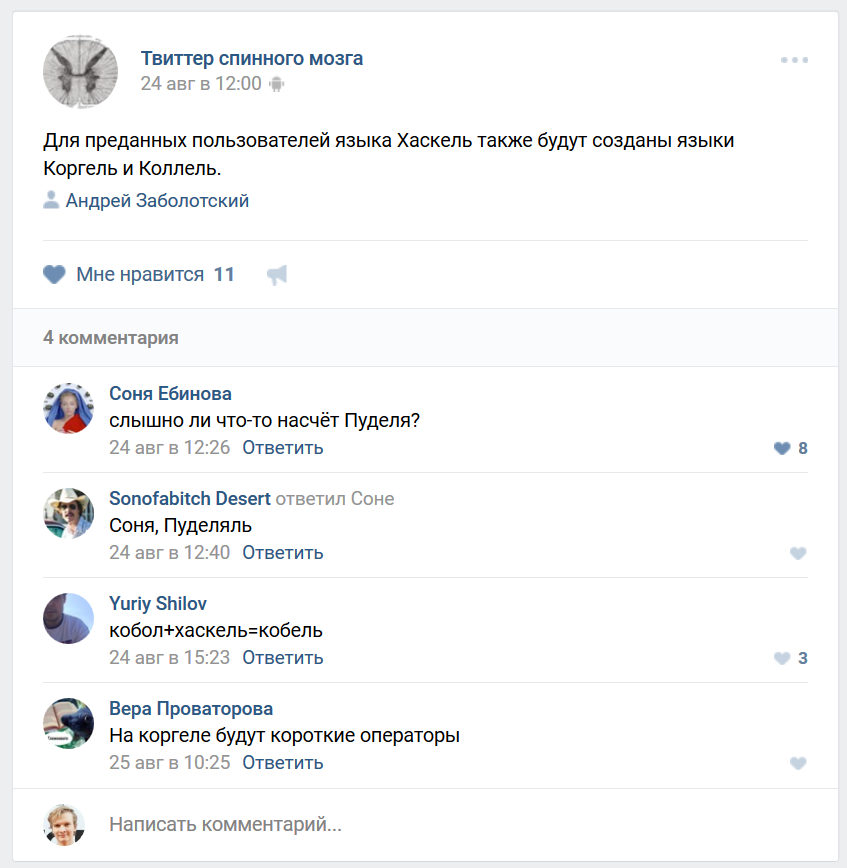
\includegraphics[scale=0.3]{twispicord-haskell.png}
	\end{center}
\end{frame}

\subsection{Функции высшего порядка}

\begin{frame}
	\tableofcontents[currentsection,currentsubsection]
\end{frame}

\begin{frame}{Напоминание}
	\begin{itemize}
		\item Функция является \textit{функцией высшего порядка}, если она в качестве одного из аргументов принимает другую функцию.
		\item Пример: \t{map}. Он первым параметром принимает функцию, которая преобразует элементы списка.
		\item Пример: \t{dropWhile}. Первый аргумент умеет по элементу сообщать, надо остановиться или нет.
		\item Пример: \t{filter cond list}. Оставляет в списке только элементы, удовлетворяющие условию.
		\item Функции высшего порядка является основными кирпичиками в функциональном программировании.
	\end{itemize}
\end{frame}

\begin{frame}[fragile]{Ещё один паттерн}
\begin{minted}{haskell}
sum (x:xs) = x + sum xs
sum _ = 0

prod (x:xs) = x * prod xs
prod _ = 1

max (x:xs) = max x (max xs)
max x = -1

concat (x:xs) = x ++ (concat xs)
concat _ = ""
\end{minted}
	Что общего?
	\pause
	\begin{itemize}
		\item Все эти функции считают функцию от множества элементов.
		\item Для пересчёта требуется знать только текущее значение и очередной элемент.
	\end{itemize}
\end{frame}

\begin{frame}[t,fragile]{Правая свёртка}
\begin{minted}{haskell}
foldr f a (x:xs) = f x (foldr f a xs)
foldr f a _ = a

sum    xs = foldr (+)  0    xs
prod   xs = foldr (*)  1    xs
max    xs = foldr max  (-1) xs
concat xs = foldr (++) ""   xs
\end{minted}
	Ещё одна популярная функция высшего порядка.
\end{frame}

\begin{frame}[fragile]{Упражнение на понимание}
\begin{minted}{haskell}
foldr f a (x:xs) = f x (foldr f a xs)
foldr f a _ = a
\end{minted}

	А что такое \t{foldr (:) [4,5] xs}?
	\pause
\begin{minted}{haskell}
foldr (:) [4,5] [1,2,3] =
1:(foldr (:) [4,5] [2,3]) =
1:(2:(foldr (:) [4,5] [3])) =
1:(2:(3:(foldr (:) [4,5] []))) =
1:(2:(3:[4,5])) =
[1,2,3,4,5]
\end{minted}
	Дописывание \t{[4,5]} в конец списка.

\begin{minted}{haskell}
(++) a b = foldr (:) b a
\end{minted}
\end{frame}

\begin{frame}{Картинка}
	\begin{center}
		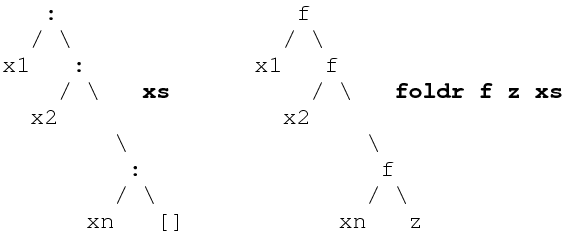
\includegraphics[scale=0.5]{foldr.png}
	\end{center}
	Бамбук растёт вправо, поэтому \textit{правая} свёртка.
\end{frame}

\begin{frame}[fragile]{Упражнения}
	Как узнать, все ли элементы равны \t{True}? \pause
\begin{minted}{haskell}
foldr (&&) True xs
\end{minted}

	Как узнать сумму квадратов чисел в массиве? \pause
\begin{minted}{haskell}
foldr (+) 0 (map (^2) xs)
\end{minted}

	Как выразить \t{map} через \t{foldr}? \pause
\begin{minted}{haskell}
map f xs = foldr (\a x -> (f a):x) [] xs
\end{minted}
	Вывод: в теории почти всё есть \t{foldr}.
	На практике лучше использовать готовые функции.
\end{frame}

\subsection{Статический полиморфизм функций}

\begin{frame}
	\tableofcontents[currentsection,currentsubsection]
\end{frame}

\begin{frame}
	\begin{itemize}
		\item Мы нигде не указывали типы ни аргументов функций, ни возвращаемых значений.
		\item Свободно использовали функции для разных типов (вроде \t{map}).
		\item Если набрать \t{:t map} в GHCI, увидим её тип:
		\[
			\t{\underbrace{(a~->~b)}_{\text{функция}}~->~\underbrace{[a]}_{\text{исходный список}}~->~\underbrace{[b]}_{\text{результат}}}.
		\]
		\item Справа от последней \t{->} "--- возвращаемое значение, до этого "--- аргументы.
		\item Тут \t{a} и \t{b} "--- типовые переменные. На их месте может стоять любой тип.
		\item Естественным образом получаем, что \t{map} вообще всё равно, с какими списками работать.
		\item Haskell автоматически выводит наиболее общие типы для практически всех функций.
		\item Все проверки типов "--- \textit{на этапе компиляции}.
	\end{itemize}
\end{frame}

\begin{frame}{Что могут делать функции}
	\begin{itemize}
		\item Что вообще может делать \textit{чистая} функция с типом \t{Bool~->~Bool}?
		\item Их всего $2^2=4$ различных: всегда \t{True}, всегда \t{False}, отрицание, тождественная.
		\item А что может делать полиморфная функция с типом \t{a~->~a}? \pause
		\item Только возвращать свой аргумент "--- она не имеет права ничего про него предполагать. \pause
		\item А функции с типом \t{a~->~b} не бывает "--- она в общем случае не может создать что-то типа \t{b}.
		\item Что может делать \t{a~->~[a]}? \pause
		\item Только создавать список из одинаковых элементов \textit{фиксированной} длины, которая не зависит от аргумента.
	\end{itemize}
\end{frame}

\begin{frame}{Игра}
	Ваша задача "--- по типу функции угадать, что она делает.
	\begin{tabular}{c|c}
		\centering
		Тип & Функция \\\hline
		\t{a -> a} & \pause\t{id x = x} \\\pause
		\t{a -> b -> a} & \pause\t{fst x y = x} \\\pause
		\t{a -> b -> b} & \pause\t{snd x y = y} \\\pause
		\t{(a -> b) -> a -> b} & \pause\t{apply f x = f x} \\\pause
		\t{[a] -> a} & \pause\t{get xs = xs !! c} \\\pause
		\t{(a -> Bool) -> [a] -> [a]} & \pause\t{filter} \\\pause
		\t{(a -> Bool) -> [a] -> [a]} & \pause\t{dropWhile} \\\pause
		\t{(a -> Int) -> [a] -> Int} & \pause\t{sum (map f xs)} \\\pause
		\t{(a -> b -> b) -> b -> [a] -> b} & \pause\t{foldr}
	\end{tabular}
\end{frame}

\begin{frame}{Вывод типов}
	Ваша задача "--- по определению функции вывести наиболее общий тип.
	\begin{tabular}{c|c}
		\centering
		Функция & Тип \\\hline
		\t{foo x y = x y} & \pause \t{(a -> b) -> a -> b} \\\pause
		\t{foo x y z = x y z} & \pause \t{(a -> b -> c) -> a -> b -> c} \\\pause
		\t{foo x y z = (x y) + (x z)} & \pause \t{(a -> Int) -> a -> a -> Int} \\\pause
		\t{foo x y = (x y) + y} & \pause \t{(Int -> Int) -> Int -> Int} \\\pause
		\t{foo x y = (x y):y} & \pause \t{([a] -> a) -> [a] -> [a]} \\
	\end{tabular}
\end{frame}

\begin{frame}{Резюме}
	\begin{itemize}
		\item Без полиморфизма функции высшего порядка были бы бесполезны.
		\item Часто по типу полиморфной функции можно догадаться, что она делает.
		\item Есть специальный поисковик \href{https://www.haskell.org/hoogle/}{Hoogle}, который ищет функции по их типу.
		\item Hoogle "--- полезная штука, если вам нужна какая-то <<очевидно полезная>> функция. Найдётся всё.
	\end{itemize}
\end{frame}

\subsection{Ленивые вычисления}

\begin{frame}
	\tableofcontents[currentsection,currentsubsection]
\end{frame}

\begin{frame}[fragile]{Идея}
	\begin{itemize}
		\item В классических языках аргументы сначала вычисляются, потом передаются функции: в вызове \t{foo(bar())} сначала вычислится \t{bar()}, а результат передадут в \t{foo()}.
		\item В Haskell наоборот: если функции неважно, что именно ей передали в качестве аргумента "--- это нечто не будет вычислено.
		\item Другими словами, вычисления производят только от плохой жизни: если по-другому никак.
		\item Например, если надо аргумент сравнить с шаблоном.
		\item В функции \t{fst} второй аргумент вычисляться никогда не будет:
\begin{minted}{haskell}
fst x y = x
\end{minted}
		\item А в функции \t{if'} будет вычислен только нужный аргумент:
\begin{minted}{haskell}
if' True  x _ = x
if' False _ y = y
\end{minted}
		\item Приходится тащить вместо невычисленного выражения инструкцию, как его получить.
	\end{itemize}
\end{frame}

\begin{frame}[fragile]{Бесконечные структуры}
	\begin{itemize}
		\item Напоминание: \t{[1, 2, 3]} "--- это сахар для \t{1:2:3:[]}.
		\item Попробуем завести бесконечный список из единиц:
\begin{minted}{haskell}
ones = 1:1:1:1:1:1:...
\end{minted}
		\item Так как бесконечную строчку написать не можем, придётся заметить рекурсию:
\begin{minted}{haskell}
ones = 1:ones
\end{minted}
		\item Этого уже хватит для вычисления, попробуйте \t{take 10 ones}.
		\item Как работает: хвост списка вычисляется только тогда, когда он реально нужен.
		\item Поэтому если никто не залез дальше второго элемента, то третий и последующие не будут вычислены, а будет просто храниться, как их можно в случае чего получить.
	\end{itemize}
\end{frame}

\begin{frame}[fragile]{Подробный пример}
\begin{minted}{haskell}
take 0 _ = []
take n (x:xs) = x:(take (n - 1) xs)
ones = 1:ones
take 3 ones = take 3 (1:ones) = 1:(take (3-1) ones)
take 2 ones = take 2 (1:ones) = 1:(take (2-1) ones)
take 1 ones = take 1 (1:ones) = 1:(take (1-1) ones)
take 0 ones = []
take 3 ones = 1:1:1:[] = [1, 1, 1]
\end{minted}
\end{frame}

\begin{frame}[fragile]{Пример похитрее}
\begin{minted}{haskell}
iota n = n:(iota (n + 1))
take 3 (iota 5) = take 3 (5:iota 6) =
5:(take 2 (iota 6)) = 5:(take 2 (6:iota 7)) =
5:6:(take 1 (iota 7)) = 5:6:(take 1 (7:iota 8)) = 
5:6:7:(take 0 (iota 8)) = 5:6:7:[]
iota n = [n, n + 1, n + 2, ...]
\end{minted}
	Практически так реализован синтаксический сахар \t{[5..]}.
\end{frame}

\begin{frame}[fragile]{Числа Фибоначчи}
	Составляем уравнение на список из чисел Фибоначчи:
\begin{minted}{haskell}
fib   = [1, 1, 2, 3, 5, 8, ...]
0:fib = [0, 1, 1, 2, 3, 5, 8, ...]
zipWith (+) fib (0:fib) = 
        [1, 2, 3, 5, 8, 13, ...]
1:zipWith (+) fib (0:fib) =
        [1, 1, 2, 3, 5, 8, ...]
fib = 1:zipWith (+) fib (0:fib)  -- Определение в Haskell
\end{minted}
\end{frame}

\begin{frame}[fragile]{Вычисление Фибоначчи}
\begin{minted}{haskell}
fib = 1:zipWith (+) fib (0:fib)  -- Определение в Haskell
\end{minted}
	\begin{itemize}
		\item Изначально знаем только \t{fib !! 0}.
		\item Когда надо вычислить \t{fib !! 1}, надо вычислить нулевой элемент от \t{zipWith}.
		\item А для этого надо знать нулевые элементы от \t{fib} и \t{0:fib}, оба знаем.
		\item Значит, их сумма и есть \t{fib !! 1}.
		\item Когда потребуется вычислить \t{fib !! 2}, надо будет вычислить первый элемент от \t{zipWith}.
		\item Для этого придётся раскрыть \t{fib} дважды (как в предыдущих пунктах), а \t{0:fib} "--- один раз.
		\item Раскрыть получится "--- это элементы мы уже считали. Значит, посчитаем их сумму и \t{fib !! 2}.
		\item И так до бесконечности.
		\item Время работы и память неизвестны :)
	\end{itemize}
\end{frame}

\begin{frame}[fragile]{Особенности бесконечных списков}
	\begin{itemize}
		\item У них нет конца.
		\item Если ваша функция пытается дойти до конца списка "--- у неё проблемы:
\begin{minted}{haskell}
getFirstTen xs = take (min 10 (length xs)) xs
length xs  -- Не работает с бесконечными списками.
\end{minted}
		\item Из-за ленивости операции над бесконечными списками реальны:
\begin{minted}{haskell}
take 0 _      = []  -- Тут второй аргумент не вычисляется
take n (x:xs) = x:(take (n - 1) xs)
\end{minted}
		\item Или даже так:
\begin{minted}{haskell}
any' (True :_)  = True
any' (_    :xs) = any' xs
\end{minted}
		\item Функции в домашнем задании должны корректно обрабаывать те бесконечные списки, на которых поведение определено.
		\item Надо писать аккуратно.
	\end{itemize}
\end{frame}

\begin{frame}[fragile]{Упражнение}
	\begin{itemize}
		\item Напишите функцию \t{concat}, который приписывает один список к другому.
		\item Работает в точности как оператор \t{(++)}.
		\item Когда осмысленно получать на вход бесконечный список?
	\end{itemize}
	\pause
\begin{minted}{haskell}
concat (x:xs) ys = x:(concat xs ys)
concat _      ys = ys
\end{minted}
	\begin{itemize}
		\item Если получаем бесконечный список как первый аргумент "--- второй не используется.
		\item Если получаем бесконечный список как второй аргумент "--- он дописывается в конец первого.
		\item В Haskell оператор \t{(++)} действительно работает за линию.
	\end{itemize}
\end{frame}

\subsection{Резюме}

\begin{frame}
	\tableofcontents[currentsection,currentsubsection]
\end{frame}

\begin{frame}
	\begin{itemize}
		\item Haskell строго типизирован и есть полиморфные функции, всё проверяется на этапе компиляции.
		\item Циклов нет, переменных нет, всё делается рекурсивно.
		\item \t{if}'ы не нужны "--- используем pattern matching, в крайнем случае "--- guards.
		\item На Haskell тоже можно как-то писать в императивном стиле.
		\item Лучше писать в функциональном стиле, комбинируя функции высшего порядка со своими.
		\item Самая мощная функция из известных нам сейчас "--- \t{foldr}.
		\item Вычисления очень ленивы: пока не потребуется сравнить с чем-то, вычисления не будет.
		\item Из-за этого возможны бесконечные структуры и разумные конечные операции с ними.
		\item Списки односвязные, из-за этого они бывают бесконечными.
	\end{itemize}
\end{frame}

\subsection{Грабли и плюшки}

\begin{frame}
	\tableofcontents[currentsection,currentsubsection]
\end{frame}

\begin{frame}[fragile]{Классы типов}
	\begin{itemize}
		\item Иногда хочется функцию полиморфную, но с ограничением на тип.
		\item Например, \t{min} должен уметь сравнивать свои аргументы.
		\item Набор свойств, которыми должен обладать тип, называют \textit{классом типа}.
		\item Подробнее разберём на следующем занятии.
		\item То, что идёт перед \t{=>} в типе в Haskell "--- это как раз ограничения на классы:
\begin{minted}{haskell}
min :: Ord a => a -> a -> a
\end{minted}
		\item \t{a} "--- любой тип, лежащий в классе \t{Ord}.
		\item Не путать с классами из ООП!
		\item Тут <<класс>> означает <<множество>>, как в математике.
	\end{itemize}
\end{frame}

\begin{frame}{Очень строгая типизация}
	% 08-01-types.hs
	\begin{itemize}
		\item Есть разные типы для вещественных и целых чисел.
		\item Оператор \t{==} между разными типами чисел не определён.
		\item Но тестом \t{2 == 2.0} это не поймать.
		\item Тип числовой константы определяется в момент компиляции: это будет либо вещественное число (класс \t{Fractional}), либо целое (класс \t{Integral}), либо любое (класс \t{Num}).
		\item Для конвертации между \t{Fractional} и \t{Integral} можно использовать \t{fromIntegral} и \t{round}.
	\end{itemize}
\end{frame}

\begin{frame}[fragile]{Каррирование}
	\begin{itemize}
		\item Функция от двух аргументов $f(x, y)$ "--- то же самое, что функция от одного аргумента $f'(x)$,
			которая возвращает функцию от одного аргумента $g_x(y)=f(x, y)$.
		\item Такой переход называется \textit{каррированием}
		\item С точки зрения Haskell, функции типов \t{a -> b -> c} и \t{a -> (b -> c)} неотличимы.
		\item Все функции в Haskell "--- от одного аргумента, остальное "--- сахар.
		\item Из-за этого частичное применение и работает: \t{(3+)} и \t{(+) 3} равны.
		\item Можно явно написать функцию от двух аргументов:
\begin{minted}{haskell}
s (a, b) = a + b
s' = uncurry (+)
\end{minted}
	\end{itemize}
\end{frame}

\begin{frame}[fragile]{Способы определения функций}
	\begin{itemize}
		\item
\begin{minted}{haskell}
addTen x = x + 10
addTenToAll x = map addTen x
\end{minted}
		\item
\begin{minted}{haskell}
addTen = (+10)
addTenToAll = map f
\end{minted}
	\end{itemize}
\end{frame}

\begin{frame}[fragile]{Композиция функций}
	Точка "--- оператор композиции функций:
\begin{minted}{haskell}
(.) :: (b -> c) -> (a -> b) -> (a -> c)
-- Приоритет низкий
((+5) . (*3)) 10
\end{minted}
	Читать надо справа налево:
\begin{minted}{haskell}
(concat . map words . lines) "1 2\n10 11\n" 
\end{minted}
	Композиции функций в каком-то смысле лучше, чем свои вспомогательные функции или явные вызовы.
\end{frame}

\begin{frame}{Унарный минус}
	\begin{itemize}
		\item Единственный унарный оператор в Haskell.
		\item Захардкожен костылями.
		\item Ломает красоту, потому что \t{(-3)} надо интерпретировать как унарный минус, а не как оператор \t{-} с зафиксированным операндом.
		\item А \t{((-)3)} надо интерпретировать, как оператор \t{(-)} с зафиксированным первым (левым) операндом.
		\item Поэтому зафиксировать правый аргумент у бинарного минуса никак нельзя, кроме лямбда-функций.
	\end{itemize}
\end{frame}

\begin{frame}[fragile]{Ввод-вывод}
	\textbf{В домашке не потребуется}
\begin{minted}{haskell}
solve :: Int -> Int
solve = (+1)
mainPure :: [String] -> [String]
mainPure = map (show . solve . (read :: String -> Int))
main = interact $ (unlines . mainPure . lines)
\end{minted}
	\begin{itemize}
		\item Функции \t{main} и \t{interact} "--- пока что магия
		\item Функция \t{show} преобразует почти любое значение в строчку
		\item Функция \t{read}, если явно указать её тип, преобразует строчку в значение
		\item Всё работает лениво и интерактивно
	\end{itemize}
\end{frame}

\section{Бонус}

\begin{frame}
	\tableofcontents[currentsection,currentsubsection]
\end{frame}

\begin{frame}{Мои наблюдения-1}
	\begin{itemize}
		\item На функциональных языках обычно очень компактные программы и много синтаксического сахара.
		\item Обычно функциональные языки (в том числе Haskell) умеют очень сильно расширять свой синтаксис до неузнаваемости.
		\item Иногда всё это превращается в сахарную вату.
		\item Элементы ФП в разной степени поддерживаются в разных языках, в том числе в
			<<императивных>>: C++, Python, Java.
		\item Есть модные смеси императивного и функционального программирования вроде Scala или OCaml.
		\item Некоторые функциональные языки используются в реальной жизни: Erlang.
		\item Чисто функциональные программы может быть сложнее отлаживать, так как нет <<состояния программы>>.
	\end{itemize}
\end{frame}

\begin{frame}{Мои наблюдения-2}
	\begin{itemize}
		\item Многие идеи из ФП полезны и в повседневной жизни:
			\begin{itemize}
				\item Неизменяемое состояние.
				\item Функции высшего порядка (где есть поддержка в языке).
				\item Чистые функции без побочных эффектов.
			\end{itemize}
		\item Если язык поддерживают хотя бы \t{map}, лямбда-функции или list comprehension,
			на нём уже намного приятнее писать.
		\item Функциональные элементы могут сильно упростить код императивной программы без потери скорости.
		\item Дополнительных проблем эти элементы не вносят.
		\item Надо быть аккуратными и не мешать их с изменяемым состоянием.
	\end{itemize}
\end{frame}
	

\section{Ссылки}

\begin{frame}
	\begin{itemize}
		\item
			\href{https://maryrosecook.com/blog/post/a-practical-introduction-to-functional-programming}{Практическое введение в функциональное программирование} "--- идеология.
		\item
			\href{http://learnyouahaskell.com}{learnyouahaskell.com}, нас интересуют главы 2 и 4-6.
		\item
			Есть перевод на русский: <<Изучай Haskell во имя добра!>>
		\item
			\href{http://camlback.cs.ucla.edu}{Проверяющая система с задачами}.
		\item
			\href{https://www.inf.ed.ac.uk/teaching/courses/inf1/fp/}{Лекции и слайды на английском}.
		\item
			\href{https://www.ohaskell.guide/whales-n-turtle.html}{Руководство на русском} (пропустите раздел с модулями).
	\end{itemize}
\end{frame}


\end{document}
